%%%%%%%%%%%%%%%%%%%%%%%%%%%%%%%%%%%%%%%%%%%%%%%%%%%%%%%%%%%%%%%%%%%%%%%%%%%%%
%% MS Draft Journal of Ecology Special Issue, Dispersal - 
%% Pedro - 07 April 2016
%----------------------------------------------------------------------------
%%%%%%%%%%%%%%%%%%%%%%%%%%%%%%%%%%%%%%%%%%%%%%%%%%%%%%%%%%%%%%%%%%%%% Headers
\documentclass[a4paper, 12pt]{article}
\usepackage{graphicx}
\usepackage[utf8]{inputenc}
\usepackage[a4paper]{geometry}
\usepackage{hyperref}
\pagestyle{plain}
\usepackage{amsmath,amssymb}
\usepackage{geometry}
\usepackage{lscape}
\usepackage{setspace}
\usepackage{verbatim}
\usepackage{graphicx}
\usepackage{epstopdf}
\usepackage{booktabs}
\usepackage{natbib}
\usepackage{longtable}
\usepackage{rotating}                                                                                    
\newcommand{\tab}{\hspace{5mm}}
\usepackage{tabularx} 
%\usepackage{multirow}
\usepackage[margin=10pt,font=small,labelfont=bf]{caption}
\usepackage[left]{lineno}
\usepackage{caption}
\DeclareGraphicsRule{.tif}{png}{.png}{`convert #1 `basename #1 .tif`.png}
\usepackage{fancyhdr} % This should be set AFTER setting up the page geometry
\pagestyle{fancy}     % options: empty , plain , fancy
\renewcommand{\headrulewidth}{0pt} % customise the layout...
\lhead{{\tiny Jordano - What is long-distance dispersal?}}\chead{}\rhead{{\tiny JEcol-2016-0422.R1}}
\lfoot{}\cfoot{\thepage}\rfoot{}
\usepackage{parskip}
\linespread{1.75}
%%%%%%%%%%%%%%%%%%%%%%%%%%%%%%%%%%%%%%%%%%%%%%%%%%%%%%%%%%%%%%%%%% Title page
\begin{document}


\title{What is long-distance dispersal? And a taxonomy of dispersal events\\
\vspace{2cm}
}

\author{MS JEcol-2016-0422.R1\\\\Pedro Jordano$^{\dag}$}

\date{Sevilla, \today}

\maketitle


\begin{spacing}{1.0}
$^{\dag}$ {\small Integrative Ecology Group, Estaci\'on Biol\'ogica de 
Do\~nana, CSIC, Avda. Americo Vespucio, s/n, Isla de La Cartuja
E-41092 Sevilla, Spain.}\\


{\small \textit{Corresponding author:} Pedro Jordano. Integrative Ecology Group, Estaci\'on Biol\'ogica de Do\~nana, CSIC, Avda. americo Vespucio, s/n, E-41092 Sevilla, Spain. Email address: jordano@ebd.csic.es}\\

\textbf{Key words}: dispersal, frugivory, plant-animal interactions, pollination, seed dispersal\\

{\small \textbf{Manuscript information: }** Words; ** Chars; ** Pages, * Figures; * Tables.}
\end{spacing}

\maketitle
\newpage

%%%%%%%%%%%%%%%%%%%%%%%%%%%%%%%%%%%%%%%%%%%%%%%%%%%%%%%%%%%%%%%%%%%% Abstract
\section*{Abstract}
\begin{linenumbers}

1. Dispersal is a key individual-based process influencing many life-history attributes, scaling up to population-level properties (e.g., metapopulation connectivity). A persistent challenge in dispersal ecology has been the robust characterization of dispersal functions (kernels), a fundamental tool to predict how dispersal processes respond under global change scenarios. Especially the rightmost tail of these functions, i.e. the long-distance dispersal (LDD) events, are difficult to characterize empirically and to model in realistic ways. \\
2. But, when is it a LDD event? In the specific case of plants, dispersal has three basic components: 1) a distinct (sessile) source, the maternal plant producing the fruits or the paternal tree acting as a source of pollen; 2) a distance component between source and target locations; and 3) a vector actually performing the movement entailing the dispersal event. Here we discuss operative definitions of LDD based on their intrinsic properties: 1) events crossing geographic boundaries among stands; and 2) events contributing to effective gene flow and propagule migration. \\
3. Strict-sense long distance dispersal involves movement both outside the stand geographic limits and outside the genetic neighborhood area of individuals. Combinations of propagule movements within/outside these two spatial reference frames results in four distinct modes of LDD. \\
4. \textit{Synthesis.} We expect truncation of seed dispersal kernels to have multiple consequences on demography and genetics, following to the loss of key dispersal services in natural populations. Irrespective of neighborhood sizes, loss of LDD events may result in more structured and less cohesive genetic pools, with increased isolation-by-distance extending over broader areas. Proper characterization of the LDD events helps to assess, for example, how the ongoing defaunation of large-bodied frugivores pervasively entails the loss of crucial LDD functions.\\

\newpage

%%%%%%%%%%%%%%%%%%%%%%%%%%%%%%%%%%%%%%%%%%%%%%%%%%%%%%%%%%%%%%%% Introduction
\section*{Introduction}

Dispersal is a key individual-based process influencing many life-history attributes and scaling up to population-level properties (e.g., metapopulation connectivity, \citealt{Cousens:2008aa}). In the specific case of plants, largely sessile organisms, dispersal has three basic components: 1) a distinct (sessile) source, the maternal plant producing the fruits or the paternal tree acting as a source of pollen; 2) a distance component between source and target locations; and 3) a vector actually performing the movement entailing the dispersal event. While realized dispersal also depends upon stages subsequent to dissemination (e.g., successful germination and seedling establishment) \cite{Schupp:1995}, the three previous components fully characterize the dispersal process per se. Therefore, plant movement differs in important natural history details from animal dispersal, yet both can be assessed within a common conceptual framework \citep[e.g., ][]{Nathan:2006aa}. Characteristically, animal-assisted plant dispersal has three distinct, highly integrated, components missing in the process of animal dispersal: the properties of the source (parental) plant, that mediate in the foraging of the animal vector (pollinator or frugivore), the intrinsic properties of the propagule, and the functional characteristics of the animal vector who performs the movement \citep{Nathan:2008fx}.    

The movement of pollen and seeds by animals and its consequences have intrigued population geneticists and field ecologists since the infancy of both research disciplines. Each has generated an impressive body of theoretical and empirical research through the past decades, yet advances have long been co-existing in ‘parallel worlds’ and the great synergistic potential of population genetics and demography for the study of plant dispersal by animals remains little explored. Knowledge gaps still having the imprint of this conceptual disconnection include the idea of long distance dispersal, and the paradoxes of forest fragmentation effects on genetic diversity \citep{Kramer:2008kg}, survival and persistence of relict tree species \citep{Hampe:2011bv}, rapid post-Pleistocene recolonization of vast continental areas in response to climate modification \citep{Clark:1998aa,Clark:1998vi}, among other persisting issues. This conceptual isolation has been exacerbated by technical difficulties for the robust characterization of dispersal events, especially those involving movement over long-distances (long-distance dispersal, LDD). LDD is a characteristically extreme event of propagule movement in any plant population, typically occurring with an extremely low probability but potentially reaching an extremely long distance. Some progress has recently been made through the fast-paced implementation of molecular tools in ecological research labs and the availability of cutting-edge technology for biotelemetry applications. But much of the population geneticist and ecologist communities remains unaware of the state of the art in each other and likely under-appreciates their potential to validate and enrich dispersal studies \citep{Jones:2008il}. In particular, LDD events remain difficult to assess, both technically- with serious methodological problems for its reliable estimation- and conceptually. Our aim here is to review the LDD concept with a specific emphasis on dispersal of plant propagules (seeds and pollen), providing an extended definition that might be helpful in the robust quantification of LDD events.   

Two main conceptual approaches have been used to assess dispersal (Fig. 1). The “forward” approach attempts to track the dispersal events away from the known sources, e.g., by tracking the movement patterns of frugivores as they leave fruiting plants after feeding (Fig. 1A). This is the main approach used in the movement ecology framework \citep{Nathan:2008fx}, with extensive application to animal movement based on the use of advanced biotelemetry. The “backward” approach attempts to reconstruct the most likely source of a dispersed propagule by inferring the sources given the propagule delivery pattern, the fecundity of potential sources, and the dispersal function (Fig. 1B), i.e., by using an inverse modeling approach. The main technical challenge in Fig. 1A is to sample enough dispersal events away from the source to be able to fully characterize the tail (LDD events) of the dispersal function. In Fig. 1B, the main challenge is to have a robust sampling scheme with propagule collectors (e.g., seed traps) and a good characterization of the potential sources to derive robust estimates of the actual sources. Both approaches are limited logistically by the difficulties to sample the vast areas required to assess LDD events from the focal source population.    

No explicit definition of what constitutes an LDD event exists. Previous approaches \citep[e.g., ][]{Nathan:2006aa,Schurr2009long} include both absolute and proportional definitions to characterize LDD events. This means providing information about the absolute distances moved by a given percentile of the events and/or providing data on the proportion of events exceeding a given distance threshold \citep{Nathan:2008is}. The exact proportional or absolute thresholds selected remain arbitrary, as no reference spatial frame is provided within the definition of LDD. This leaves the consideration of LDD as an extreme form of context-dependent phenomenon, strongly dependent upon the scale of the biological process studied \citep{Kinlan:2005fb} and of the specific organism considered. For example, \cite{Kinlan:2005fb} used a spatial reference frame to characterize LDD events of marine organisms, where sedentary adults and larvae differ enormously in the spatial scales of their dispersal \citep{DAloia:2013fc}. Therefore, any measure of extent and reach of LDD events requires reference to an explicit spatial frame or "local" scale \citep{Kinlan:2005fb}.

We aim at providing a general framework for the quantitative analysis of LDD events so that estimates of their frequency and extent could be comparable across different study systems. We argue that both demographic and genetic elements are needed for this framework, most likely requiring a combination of field-based movement data and genetic analyses. These elements can be overlaid on previous definitions based on absolute and proportional characterizations of LDD. We start with a definition of LDD events within a spatially-explicit mechanistic framework allowing an unambiguous meaning for setting long-distance thresholds. We then use a case study to assess differential contributions of animal frugivores performing LDD.

Long-distance dispersal is currently one of the most debated topics in dispersal ecology; it defines the connectedness within the network of local populations and the possibilities for range expansion and successful colonization events. We propose a first demogenetically-based, operational definition of what a long-distance dispersal event actually is, and review existing empirical literature on distance thresholds from population and genetic perspectives. We also show how molecular tools have been used to identify the respective contributions of different animal species to the LDD portion of dispersal kernels of pollen and seeds by setting empirically-derived distance thresholds. Finally, we highlight potential applications of molecular markers beyond the quantification of just the dispersal distances that prevails in current studies, e.g., experimental approaches to assess dispersal limitation and Janzen-Connell effects.


\subsection*{LDD within a demo-genetic perspective: a taxonomy of dispersal events}

Here we propose an explicit definition of LDD and what constitutes a LDD event. Previous definitions of dispersal patterns emphasized only their distance components and characterized LDD events basically in terms of geographic distance between a dispersed propagule (or an established early seedling) and its most likely maternal or paternal (in case of pollen) source. Absolute and proportional definitions for the LDD events have been proposed depending on arbitrary thresholds of either the distance beyond which a dispersal event is LDD or the proportion of events occurring beyond a specific distance \citep{Nathan:2005jc, Nathan:2008is}. Thus, two key biological aspects of LDD events involve the transport of propagules outside a reference area: moving away from the source stand or population, and moving away from the area where relatives stand \citep{Kinlan:2005fb}. These two movements do not necessarily concur: a propagule may move over a very long distance yet still be disseminated within the reach of the neighborhood where parental individuals mate. Within a demo-genetic framework it is easy to envision a combination of situations concerning the spatial scale of the dispersal processes (Table 1) and unambiguously define different types of LDD events. The idea that dispersal occurs in reference to these two spatial reference frames, i.e., the population or stand and the genetic neighborhood area, is motivated by the fact that dispersal entails the movement of both an individual propagule (i.e., a pollen grain or a seed) and a distinct set of genes (i.e., the male genotype in case of pollen, or a seed genotype). Thus, dispersal entails simultaneous demographic and genetic effects through recruitment of new individuals in the population and through contributions to gene flow \citep{Harper:1977aa}. When considered its combined influence on demography and population genetics, the concept of LDD nicely bridges these two paradigms embedded in the biological definition of population \citep{Waples:2006ev}. 
 
Two important components of plant dispersal ecology concern the movement of propagules away from the source population, a type of dispersal relevant to colonization ability and range expansion \citep{Howe:2004}, and the movement away from the location of close relatives, i.e., a movement away from the genetic neighborhood \citep{Hardesty:2006lr,Jones:2008il}. If we classify dispersal events according to these two spatial frameworks (Table 1) we end up with four distinct types of events depending on whether or not dispersed propagules are disseminated within these reference areas. Setting the limits of a population can be problematic \citep{Waples:2006ev} yet we can identify with relative ease the geographical limits of plant stands, patches, habitat spots or other types of habitat or microhabitat discontinuities that determine landmark boundaries of biological significance \citep[see][for further discussion of boundaries for dispersal]{Kinlan:2005fb}. These "frontiers" set biological limits to what a LDD event is in relation to the geographic limits of the source population. Most plants are distributed as clumped patches, discrete stands, or relatively isolated populations, so we may distinguish between short-distance and long-distance dispersal events that end up with dissemination within or beyond, respectively, the stand or population geographic boundaries (Table 1, $SDD_{loc}$ or $LDD_{loc}$) (Figure 2).  

A second consideration in terms of spatial boundaries, with effects on dispersal patterns, is the genetic neighborhood area $N^b_e$, i.e., the spatial extent including a subset of panmictic individuals within a population \citep{Wright:1943aa,Wright:1946aa}. Thus, the $N^b_e$ area can be equal to the whole extent of the population whenever the population is unstructured and there is evidence for random mating events among all the individuals. However, most populations and stands of long-lived trees show highly aggregated and clumped distributions \citep{Seidler:2006hx}, where relatively long distances may separate groups of individuals within the same population. In these cases we might expect $N^b_e$ area to be substantially smaller than the total population area. Therefore, at least four possible scenarios exist with distinct implications in terms of consequences for dispersal (Table 1). In the case of dispersal events not extending beyond the geographic limits of the population or reference area, actual LDD events may involve dissemination beyond a reduced neighborhood area that is smaller than the geographic extent of the population, originating local long-distance ($LDD_{loc}$) dispersal events (Table 1, Fig. 2A). Actual short-distance dispersal would then involve those situations where the propagule is disseminated within \textit{both} the population limits and the genetic neighborhood boundary ($SDD_{loc}$). Along a similar reasoning, dispersal events outside the population limits will not necessarily convey LDD (Table 1, Fig. 2B): this is expected in cases where the genetic neighborhoods are extensive, going beyond the geographic limits of local populations, as in fig trees \citep{Nason:1998aa}, generating LDD events within the genetic neighborhood ($LDD_{neigh}$). Finally, strict-sense LDD events would involve dissemination outside \textit{both} the population limits and the genetic neighborhood boundary ($LDD_{ss}$) (Table 1, Fig. 2A).

While both $SDD_{loc}$ and $LDD_{loc}$ can be crucial for assuring the local persistence of populations, $LDD_{neigh}$ and $LDD_{ss}$ would be extremely important contributors to the structuring of genetic pools, realized gene flow, and maintaining connectivity in metapopulation scenarios. We argue that both the demographic and the genetic references are relevant for a proper definition of LDD.
 


\subsection*{Individual and Population Neighborhoods as Reference}

Continuous populations can be modeled with the concepts of isolation by distance and neighborhood size\citep{Wright:1943aa,Wright:1946aa}. The former refers to the case that limited gene dispersal in continuous populations produces demes that are panmictic internally, but are isolated to some extent from adjacent demes. Each group of reproducing individuals is the neighborhood, defined as the population of a region in a continuum, from which the parents of individuals born near the center may be treated as if drawn at random \citep{Wright:1969mb}. The importance and influence of the dispersal process in determining the size of the neighborhood is given by this equation, which shows how the spatial dispersion (pattern of spatial distribution) of the population influences the effective population size. This influence on the effective size is given by:  

\begin{equation}
					N^b_e= 4 \pi \sigma \delta
\end{equation}

where $\delta$ is the density of adults per unit area and $\sigma$ is the standard deviation of the distance between birth and breeding sites. This formulation is often called the neighborhood size and assumes a normal distribution of distances between parents and offspring (out in a perfect circular shape from the source). Thus, changes in the variance of dispersal distance can affect $N^b_e$ (highly clumped populations will have reduced $N^b_e$). This is the basic model of "Isolation by Distance" proposed by   \citet{Wright:1943aa,Wright:1946aa}. Under this type of model, migration (gene flow) is given by the variance in dispersal, and not by the proportion of the population that is composed of migrants (denoted $m$), as is the case with island models \citep{Slatkin:1985qb}. With enough distance separating them, two plant individuals have a low probability of mating and can be considered members of distinct genetic populations even if they are not located in geographically distinct populations.

For plants, gene flow may be accomplished by both seeds and pollen, so the variance may be decomposed to account for different patterns of seed and pollen dispersal, and to take into account the mating system (outcrossing rate, $t$). Thus, neighborhood size can be defined with the following equation (Crawford 1984) :

\begin{equation}
  		N^b_e = 4 \pi (\sigma^2_s + \frac{t \sigma^2_p}{2}) \delta (1 + t)
\end{equation}

where $\sigma_s$ is the standard deviation of seed dispersal distance, $\sigma_p$ is the standard deviation of pollen dispersal distance, and $\delta$ is the density of potential parents.

Neighborhood size in plants can be estimated by marking pollen and seeds with fluorescent dyes, tags, or stable isotope enrichment \citep{Carlo:2009wa}. However, these methods do not measure effective pollen or seed movement, but they may be combined with genetic analysis to assess genetic identity and relatedness with hypervariable DNA markers \citep{Levin:1988fm,Nason:1998aa,Godoy:2001} to achieve reliable estimates of both effective population size and neighborhood area. 

The extent of neighborhood area in plants can be extremely variable, depending on life-history attributes such as life-span, spacing patterns, mating system, etc. Even a limited sample of available information (Table S1) highlights the fact that the size of neighborhood areas can in some cases exceed the geographic limits of local populations \citep{Nason:1998aa}. The size of neighborhood areas may encompass at least four orders of magnitude, $10{^-2}-10^2$ km in radius, and include many individuals. Therefore, reference to this "genetic/evolutionary" paradigm and reference to the geographic boundaries \citep[sensu][]{Waples:2006ev} may be instrumental to understand the actual role of LDD events in shaping the structuring of genetic pools and contributing to gene dispersal. 

Whenever there is a large discrepancy between population area extent and $N^b_e$ we might expect the frequency of $LDD_{loc}$ and $LDD_{neigh}$ differ enormously. For example, relatively small $N^b_e$ may rise the importance of $LDD_{loc}$ in preserving scenarios of panmixia within a local population, as most distant dispersal events will disseminate seeds outside the neighborhood of maternal plants.


\subsection*{Empirical analysis of contributions to LDD}

Empirical evaluation of differential contributions to the different forms of LDD events outlined in Table 1 requires identification of source trees as well as assignment of the dispersed propagules to specific vectors or functional groups of vectors \citep{Jordano:2007}. Recently, DNA-barcoding techniques have been developed and successfully applied to the identification of frugivore species contributing to specific seed dispersal events whose source can be identified with genetic, direct assignment techniques \citep{GonzalezVaro:2014ij}. Otherwise, visual identification can reliably assign the genotyped seeds to frugivore species groups based on specific characteristics of scats and regurgitations \citep{Jordano:2007}. 

We inferred the frugivore groups contributing dispersal events by visually identifying scats and regurgitations in seed traps and line transects \citep[see ][ and Suppl. Mat. for additional details of methods]{Jordano:2007}. These frugivore functional groups include up to 38 bird and 4 mammal species feeding on \textit{P. mahaleb} fruits \citep{Jordano:2000ft}. Here, we differentiate four major frugivore groups: large carnivorous mammals (such as foxes, badgers, and stone martens); two species of medium-sized frugivorous birds, mistle thrushes (\textit{T. viscivorus}), and carrion crows (\textit{Corvus corone}); and a pool of small-sized frugivorous birds, including warblers, redstarts, and robins \citep{Jordano:2007}.  

To a large extent, short-distance dispersal events (strict-sense, $SDD_{loc}$ events) are contributed by small- and medium-sized (\textit{Turdus}) frugivorous birds (Table 2). Given the relatively reduced $N^b_e$ area of \textit{P. mahaleb} (Suppl. Mat. Table S1), $< 1km^2$, well below the extent of the local study population \citep{Garcia:2007he,Garcia:2005fu},  we cannot estimate $LDD_{neigh}$ events (Table 2), as all LDD events outside the reference population occur, by definition, outside the $N^b_e$ area. Larger frugivores such as corvids and the pigeon \textit{Columba palumbus} contribute most LDD events, and most immigrant seeds potentially dispersed from other populations (Fig. S2). Notably, strict-sense long-distance dispersal ($LDD_{ss}$) appears consistently associated with large-bodied frugivores (Table 2), most likely associated with a greater frequency of movements outside the local population (Fig. 4).

Empirically mapping of dispersal events for either pollen or seed disseminated by animals may result in a complex pattern of different combinations of dispersal events (Fig. S1), as animal movements are overlaid onto plant populations occupying complex landscapes, resulting in different types of SDD and LDD events. 


%%%%%%%%%%%%%%%%%%%%%%%%%%%%%%%%%%%%%%%%%%%%%%%%%%%%%%%%%%%%%%%%%% Discussion
%\section*{Discussion}

\subsection*{Long-Distance Dispersal: the ecology of extreme events}

Long-distance dispersal (LDD) is a major component of the population dynamics, genetic structure, and biogeographic history of plant species. It determines the colonization ability of new habitats and the possibilities for fragmented populations to sustain a cohesive metapopulation by immigration-emigration dynamics that rely on LDD events \citep{Nathan:2008is,Schurr2009long}. Yet our current understanding of the extent, frequency, and consequences of LDD is very limited. On one hand, theoretical models fail to predict accurately the behavior of the tail of the dispersal functions, and thus fail to predict very basic properties of LDD. On the other hand, we still have very limited documentation of actual LDD events in natural populations and we still see LDD as a sporadic, rarely far-reaching process still marked with the stamp of natural history curiosity.

Combining spatially-explicit references to the geographic population limits and the genetic neighborhood area extent ($N^b_e$) helps avoiding some imprecision in setting distance thresholds to characterize LDD events \citep{Jones:2008il}. In addition, the framework outlined in Table 1 bridges the combined demographic and genetic effects of LDD events. When methods available to assign frugivore taxa to the analyzed dispersal events, as in the study case with \textit{P. mahaleb}, a classification in the four categories of events is possible. 

The frugivore assemblage of \textit{P. mahaleb} is composed by a diversified set of animal species spanning a wide size range, ca. 12-14000 g in body mass. We might expect that this extreme variation translates in an ample pattern of foraging modes, movement distances, and fruit/seed processing \citep{Jordano:2000ft}. If the results for \textit{P. mahaleb} are generalizable to other disperser assemblages, it seems that the functional roles of frugivore species in terms of contributions to LDD events are structured in two distinct groups: small-bodied frugivores, with substantial contributions to SDD events, and large-bodied species with a disproportionate contribution to LDD events. Both components of this sort of diplochorous \citep{vanderWall:2004hv} dispersal system are very frequent in fleshy-fruited plants with diversified frugivore assemblages \citep{Galetti:2013jv}. In such cases, small-bodied frugivores largely contribute the short-distance dispersal key to support \textit{in situ} recruitment and population persistence. Yet the large-bodied frugivores distinctly contribute LDD events that sustain the connectivity of metapopulation scenarios \citep{Urban:2001}. As shown in Table 1, SDD and LDD events can be more complex when we consider the contributions to gene flow via seed and the consequences in terms of structure and spatial distributions of the genetic pools. For example, local, within-population, dispersal events may vary enormously in terms of genetic effects and local structuring of the genetic pools depending on whether they specifically contribute $SDD_{loc}$ or instead, $LDD_{loc}$. Note that only the latter actually contribute erasing any form of local genetic structure by contributing to increased genetic neigborhoods.

A number of classic studies have demonstrated that the activity of large furgivores may also significantly contribute to SDD events and inefficient dispersal because of, i.e., territorial defence, short gut retention times relative to on-tree foraging, frequent revisitation of same trees and perches, etc., resulting in substantial SDD events \citep{Pratt:1983gf,Pratt:1984ly,Snow:1984ul,Snow:1988ve,Wheelwright:1991qf}. Yet these large-bodied frugivores are crucial for both $LDD_{loc}$ and $LDD_{ss}$, given that extensive movement patterns and extremely large foraging ranges may frequently contribute dissemination beyond distance thresholds defined with either spatial landscape or genetic references. Recent analyses of the movement ecology of large frugivores, coupled with results of their seed dispersal services emphasize that LDD are by no means exceptional, either in terms of frequency and extent \citep[e.g., ][]{Westcott:2005,Bueno:2013cg,Morales:2013dg,Carlo:2013vd}. In addition, medium-sized birds such as thrushes (\textit{Turdus} spp.) can contribute substantial $LDD_{loc}$ events, i.e., local LDD events contributing to erase local population genetic structuring, effectively increasing the size of genetic neighborhoods. In the case of \textit{P. mahaleb} up to 55.49\% of their dispersal events are $LDD_{loc}$ events. These birds are efficient seed dispersers of \textit{P. mahaleb} and other fleshy-fruited species \citep{Snow:1988ve,Jordano:2000ft,Carlo:2013vd}, also showing significant contributions of $LDD_{ss}$ events.

As defined in our framework (Table 1), LDD, and in particular $LDD_{ss}$ events are a specific case of extreme events \citep{Garcia:2017aa} consistently associated with large-sized frugivores, yet including also medium-sized and highly efficient frugivorous bird species. Robustly characterizing the expected frequencies and extent of those extreme events would be crucial to properly assess the functional role of frugivores and the full range of influences (demographic, genetic) in plant populations.


\subsection*{Challenges and future avenues for research}

Pollen and seed dispersal in plants are essentially spatially-structured processes for which the outcomes of interactions with dispersal vectors is intimately linked to landscape features. Given this mechanistic link between the features of the vector and the environments where its displacement occurs \citep{Nathan:2008fx}, consideration of landscape is key to understand the consequences of LDD events. Yet these consequences hit two central aspects of plant life-histories: the demographic recruitment process \citep{Harper:1977aa}, and the genetic signatures of pollen- and seed-mediated gene flow in complex landscapes \citep{Sork:1999}. Recent evidences point out that the selective extinction of large-bodied frugivores may significantly impact plant populations dependent on frugivores both in terms  of recruitment \citep{Traveset:2012he,PerezMendez:2015hya} and genetic connectivity \citep{Perez-Mendez:2016dz}. Frugivore downsizing represents a lasting challenge for the collapse of seed dispersal processes where $LDD_{ss}$ events are crucial for population persistence and the cohesion of fragmented populations within metapopulation scenarios.

We advocate \citep[also see ][]{Jordano:2002tr,Nathan:2003qe,Jones:2008il,Hardesty:2011jn} a combination of approaches including large-scale biotelemetry to characterize animal movement, coupled with large-scale genetic sampling of dispersed propagules, and demogenetic approaches that combine both demographic and genetic research. A crucial aspect would be to effectively associate the role of individual frugivore species to specific dispersal outcomes, by identifying the actual disperser contributing a dissemination event \citep{GonzalezVaro:2014ij} and simultaneously characterizing the source maternal plant \citep{Jordano:2002tr}.

The actual challenges to properly characterize the typologies of LDD events outlined in Table 1 will probably persist. We need more efficient quantitative approaches to assess these infrequent events, that occur over enormous spatial scales and that need to be documented with sample sizes sufficient to facilitate modeling efforts and robust statistical inferences. These are not trivial difficulties given the urgency to assess how forest loss, defaunation, genetic purging due to logging, etc., alter plant populations. 




\newpage

%%%%%%%%%%%%%%%%%%%%%%%%%%%%%%%%%%%%%%%%%%%%%%%%%%%%%%%%%%%% Acknowledgements
\emph{Acknowledgements}. I am indebted to Cristina García, José A. Godoy, Manolo Carrión, Juan Luis García-Castaño, Jesús Rodríguez and, especially, Juan Miguel Arroyo for generous help with field and laboratory work and making possible this study. I appreciate the help and advice of Cristina García and Etienne Klein during the final stages of the manuscript. The study was supported by a Junta de Andalucía Excellence Grant (RNM-5731), as well as a Severo Ochoa Excellence Award from the Ministerio de Economía y Competitividad (SEV-2012-0262). The Agencia de Medio Ambiente, Junta de Andalucía, provided generous facilities that made possible this study in the Andalusian natural parks (Sierra de Cazorla, Alcornocales) and authorized my work there.

\end{linenumbers}

\newpage

%\section*{References}
%%%%%%%%%%%%%%%%%%%%%%%%%%%%%%%%%%%%%%%%%%%%%%%%%%%%%%%%%%%%%%%%%%%%%%%%%%%%% References
%%% Unnumbered Literature Cited
\bibliographystyle{bes}        %Compile with bes.bst style file
\bibliography{MS_BES}

%%%%%%%%%%%%%%%%%%%%%%%%%%%%%%%%%%%%%%%%%%%%%%%%%%%%%%%%%%%%%%%%%%%%% FIGURES

\newpage

%%%%%%%%%%%%%%%%%%%%%%%%%%%%%%%%%%%%%%%%%%%%%%%%%%%%%%%%%%%%%%%%%%%%%% TABLES
%-------------------------------------------------------------------- Table 1
\pagestyle{empty}
\begin{landscape}
	%%%%%%%%%%%%%%%%%%%%%%%%%%%%%%
%	\oddsidemargin  0.0in
%	\evensidemargin 0.0in
%	\textwidth      8.5in
	\headheight     3cm
%	\topmargin      0.0in
%	\textheight=8.0in
	%%%%%%%%%%%%%%%%%%%%%%%%%%%%%%
\begin{table}
\captionsetup{width=20cm}%.75\textwidth}
\caption{Types of dispersal as a function of population area limits and genetic neighborhood limits. See Fig. 2 for a graphical representation of the four scenarios.}
\vspace{0.5cm}
  \begin{tabular}{lcc}
    \hline
\\&Population geographic limit    &  \\\\
Genetic neighborhood limit     &Within &Outside \\\\
    \hline
\\Within  &  Local, short-distance dispersal, $SDD_{loc}$  
          &  Within neighborhood, long-distance dispersal, $LDD_{neigh}$ \\\\
Outside   &  Local, long-distance dispersal, $LDD_{loc}$    
          &  Strict sense long-distance dispersal, $LDD_{ss}$\\\\ 
    \hline
  \end{tabular}
\end{table}
\end{landscape}

\newpage

%-------------------------------------------------------------------- Table 2
\pagestyle{empty}
\begin{landscape}
\begin{table}
\captionsetup{width=21cm}%.75\textwidth}
\caption{Relative frequencies of \textit{Prunus mahaleb} seed dispersal events for different frugivore groups according to population area limits and genetic neighborhood limits. See Fig. 2 for a graphical representation of the four scenarios. \textit{N}= 655 seeds \citep[see Table 1 in ][]{Jordano:2007}. Given that the estimated neighborhood size is smaller than population area, $LDD_{neigh}$ would be zero.}
\vspace{0.5cm}
    \begin{tabular}{lp{3cm}p{3cm}p{3cm}p{3cm}p{3cm}}
    \hline \\
    Frugivore group & Within-population, within-neighborhood $SDD_{loc}$ & Within-population, long-distance $LDD_{loc}$ & Outside-population, within-neighborhood $LDD_{neigh}$ & Strict-sense long-distance $LDD_{ss}$ & \textit{N} seeds  \\\\ \hline \\
	Small-birds	    & 0.7842 &  0.0171 & 0.00 & 0.1986 & 292  \\
	\textit{Turdus} & 0.2370 &  0.5549 & 0.00 & 0.2081 & 173  \\
	Large-birds     & 0.0435 &  0.3913 & 0.00 & 0.5652 &  23  \\
	Mammals         & 0.0120 &  0.2455 & 0.00 & 0.7425 & 167  \\\\
\hline
    \end{tabular}
\end{table}
\end{landscape}

%----------------------------------------------------------------------------
 
\newpage 
 
%%%%%%%%%%%%%%%%%%%%%%%%%%%%%%%%%%%%%%%%%%%%%%%%%%%%%%%%%%% LANDSCAPE FIGURES
%%%% Figure LEGENDS
%%%% This is for sideways figures (landscape), with legend in a separate page.
\section*{Figures}
\begin{linenumbers}

\textbf{Figure 1}. The two approaches used in analyses of dispersal processes in plants. A, the “forward” approach attempts to track the dispersal events away from the known sources, e.g., by tracking the movement patterns of frugivores as they leave fruiting plants after feeding. B, the “backward” approach  attempts to reconstruct the most likely source of a dispersed propagule by inferring the sources given the propagule delivery pattern, the fecundity of potential sources, and the dispersal function. The main technical challenge in A is to sample enough dispersal events away from the source to be able to fully characterize the tail (long-distance dispersal, LDD, events) of the dispersal function. In B, the main challenge is to have a robust sampling scheme with propagule collectors (e.g., seed traps) and a good characterization of the potential sources to derive robust estimates of the actual sources with inverse-modeling techniques.\\
 
\textbf{Figure 2}. Schematic representation of different types of long-distance dispersal events in relation to the geographical limits of local populations (dashed lines) and the genetic neighborhood area $N^b_e$ (grey area) of specific individual plants (squares). Dispersal events (arrows) can be classified depending on their actual incidence on propagule movement outside these spatially-explicit reference areas (Table 1). Strict-sense long-distance dispersal events ($LDD_{ss}$) just include the LDD events that disseminate propagules out of \textit{both} the population and genetic neighborhood boundaries. A, the neighborhood area is included within the geographic limits of the population, with some dispersal events potentially contributing local LDD; B, the neighborhood area is much larger than the geographic limits of the population.\\
 
\textbf{Figure 3}. Empirical frequency distributions of seed dispersal events as a function of dispersal distance by animal frugivores consuming \textit{Prunus mahaleb} fruits. In red, left (inset), frequencies of within-population dispersal events inferred from direct assignment based on seed endocarp genotypes and maternal trees genotypes. Larger frame, left, contributions of four functional frugivore groups (small birds, medium- and large-sized birds, and mammals) to seed dissemination and proportional contributions (right bar) to dispersal of the inferred immigrant seeds (i.e., those not matching any maternal tree in the study population) \citep{Jordano:2007}.\\
 
\textbf{Figure 4}. Differential contributions of functional groups of frugivores to the four combinations of \textit{Prunus mahaleb} seed dispersal events outlined in Table 1. These result from dissemination within (yellow) or outside (blue) the population geographic limits; within-population dispersal events can either be short-distance ($SDD_{loc}$) or local LDD ($LDD_{loc}$) depending on the size of the genetic neigborhood. Dispersal outside the local population can entail short-distance dispersal, if within the genetic neighborhood area limits ($SDD_{neigh}$) (yellow) or represent strict-sense LDD ($LDD_{ss}$) (blue).\\ 
\newpage

%------------------------------------------------------------------- Figure 1
\pagestyle{empty}
\begin{figure}[htbp]
\centerline{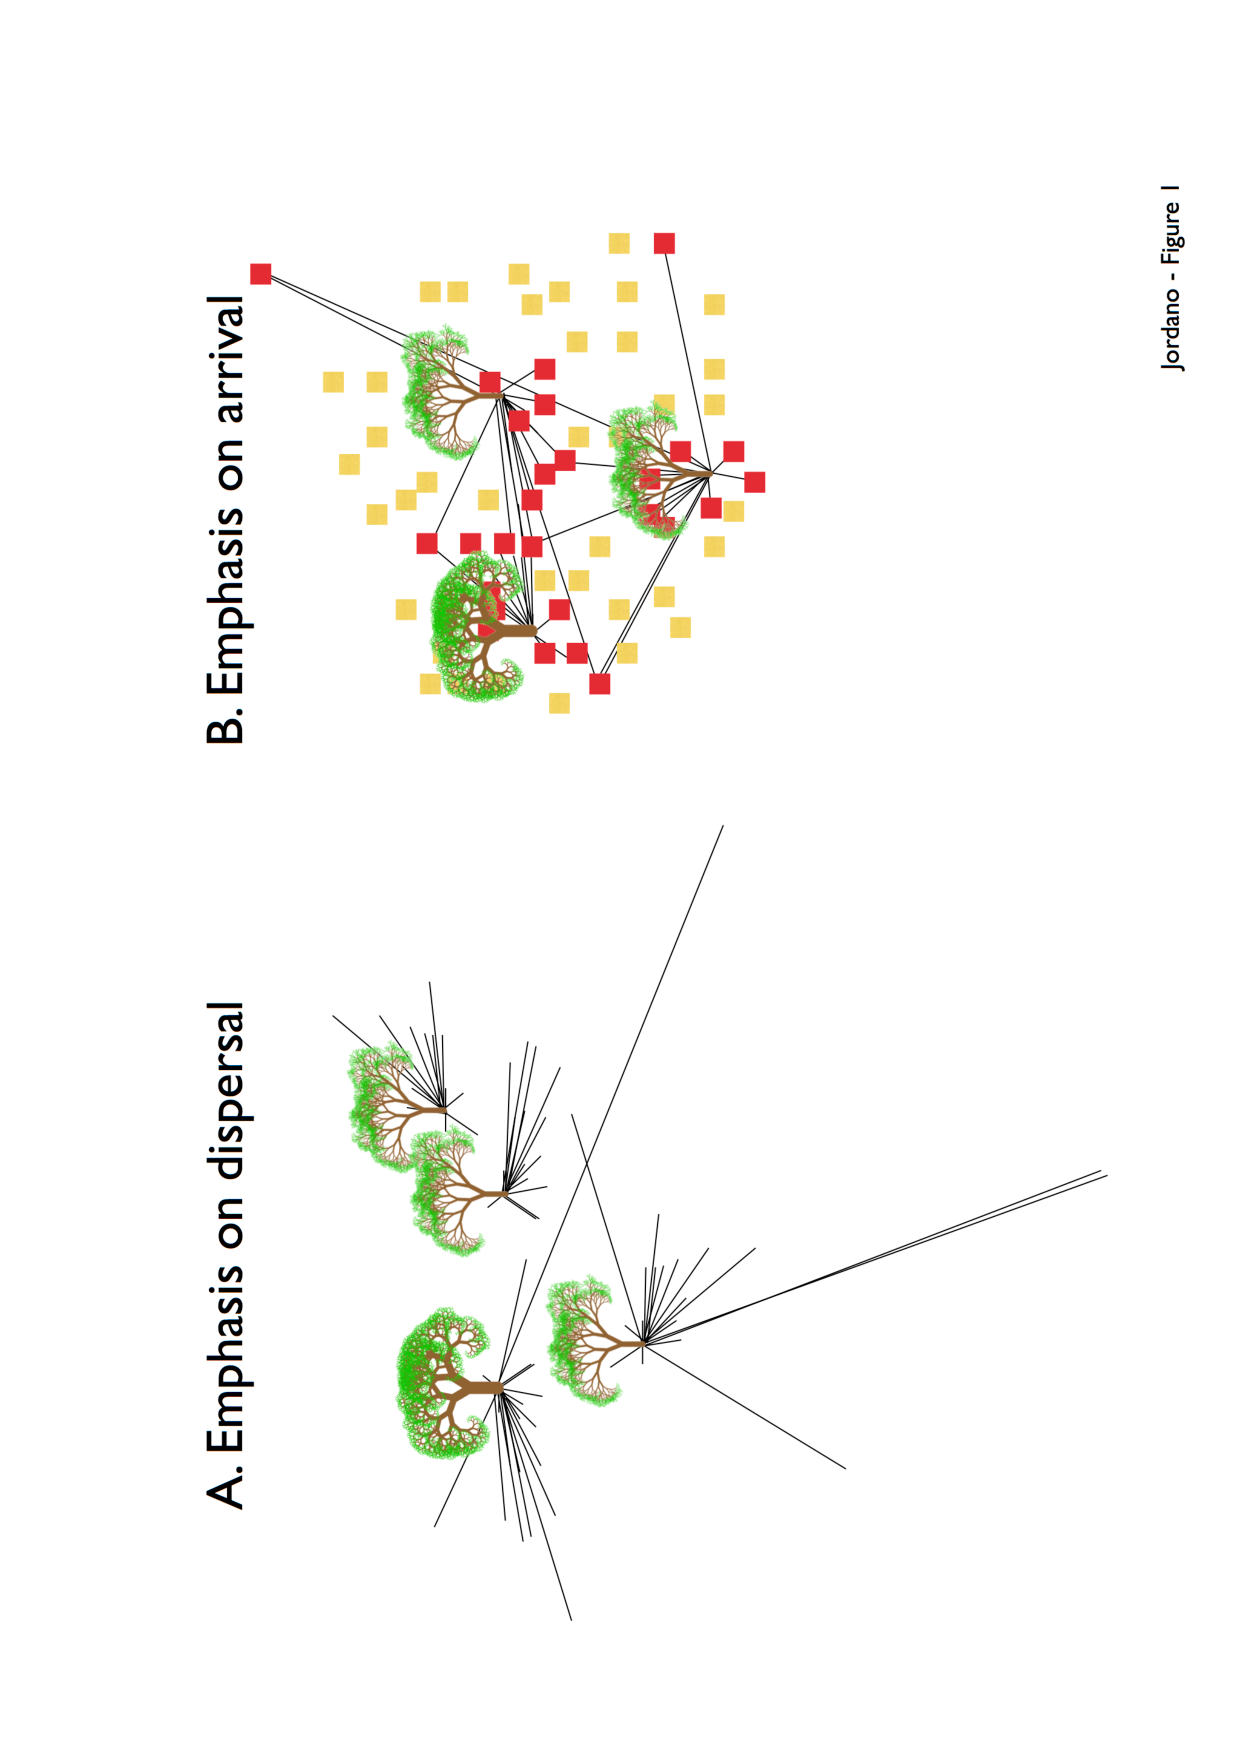
\includegraphics[height=25cm]{Fig1.pdf}}
%
%\caption{***}
\end{figure}

\newpage 
%------------------------------------------------------------------- Figure 2
\pagestyle{empty}
\begin{figure}[htbp]
\centerline{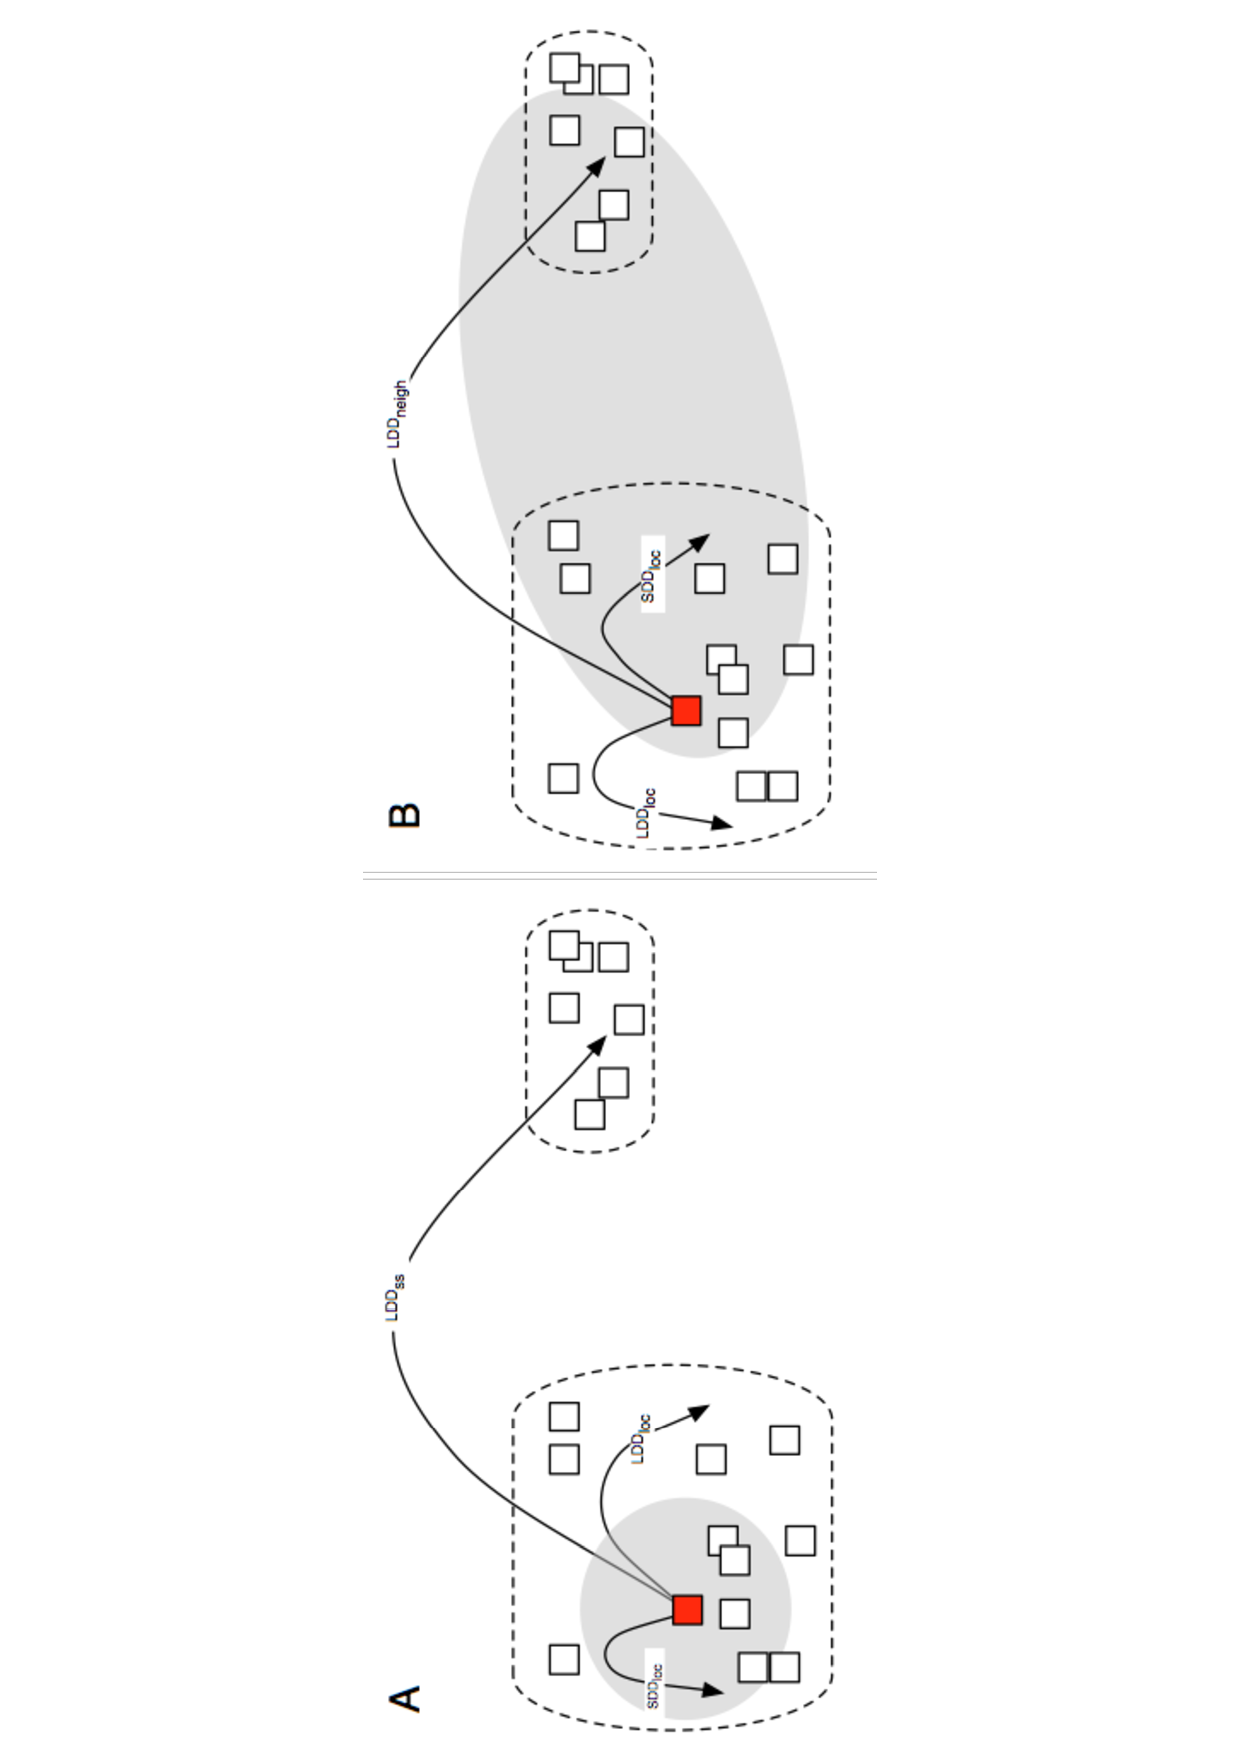
\includegraphics[height=25cm]{Fig2.pdf}}
%
%\caption{***}
\end{figure}

\newpage 
%------------------------------------------------------------------- Figure 3
\pagestyle{empty}
\begin{figure}[htbp]
\centerline{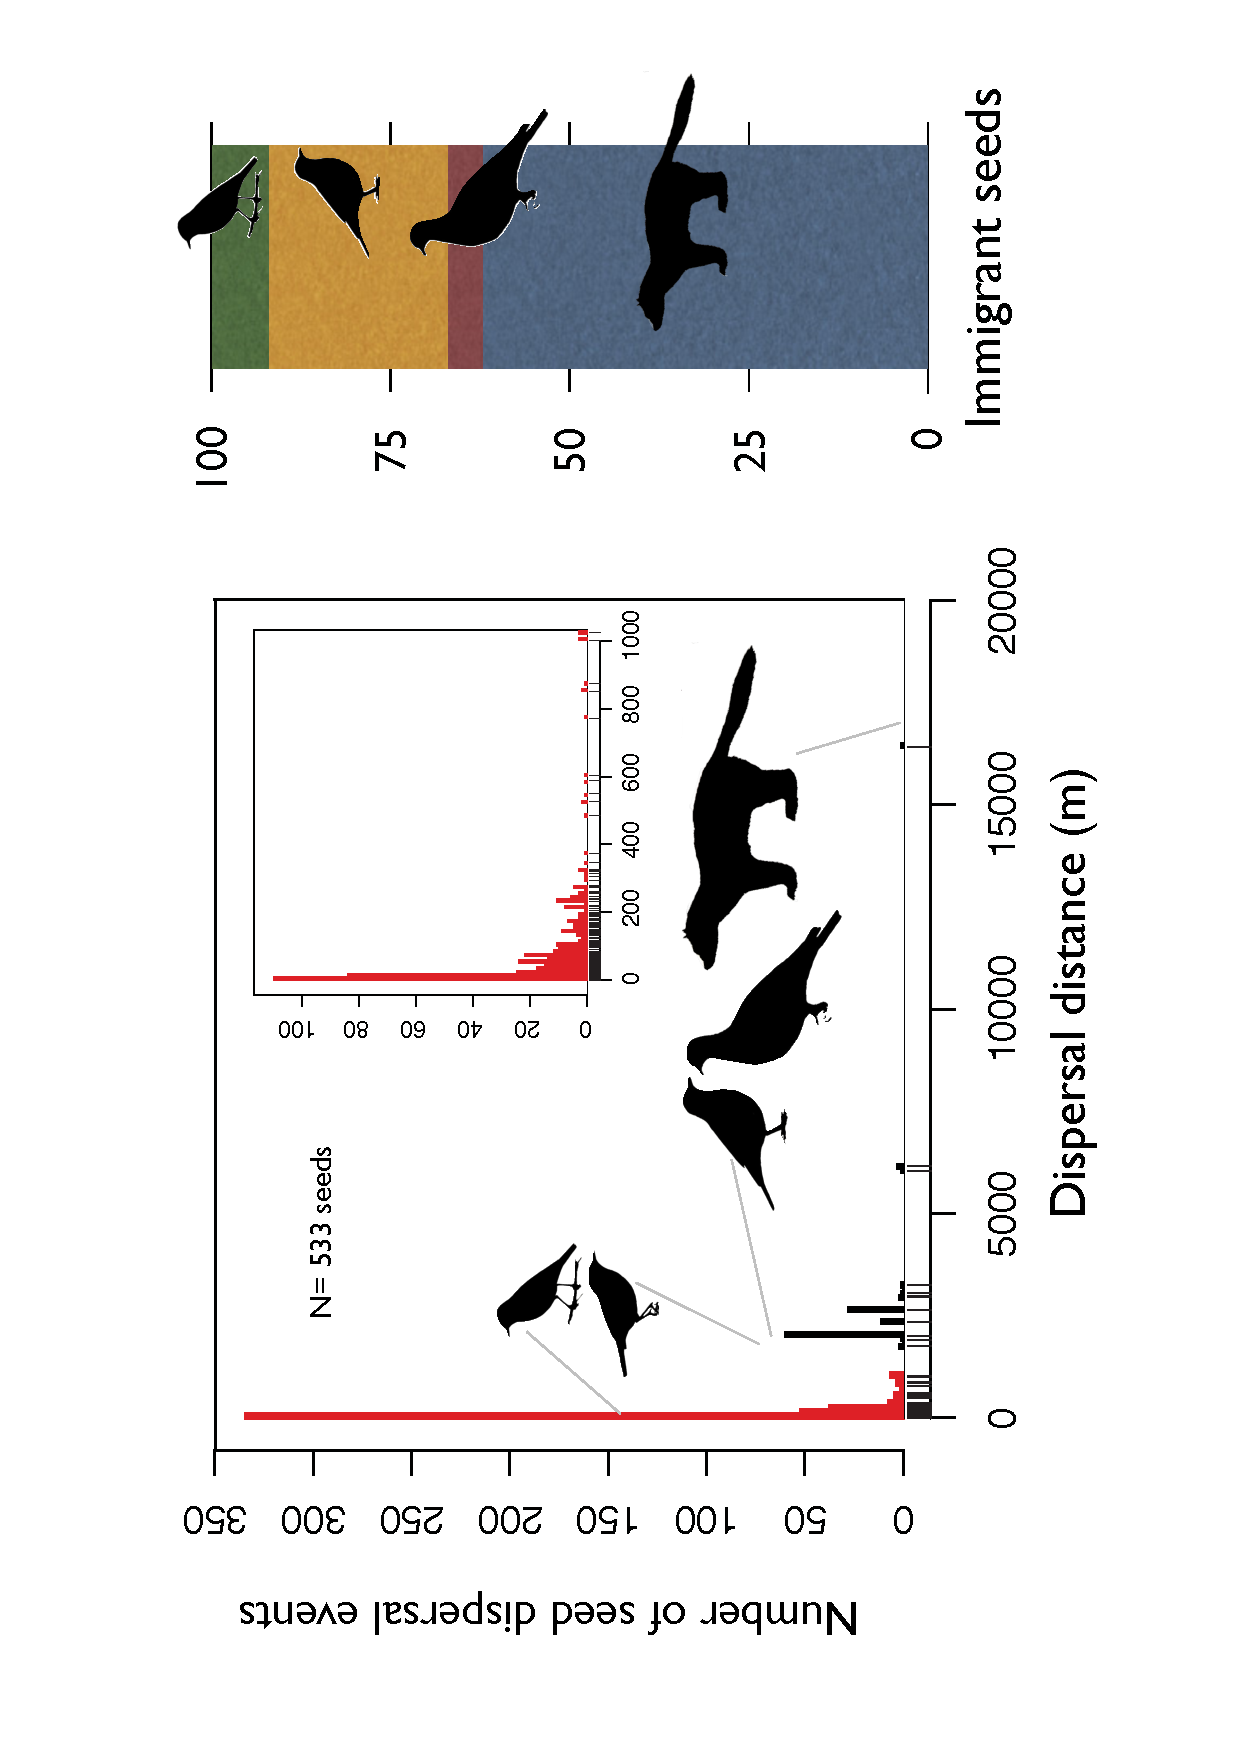
\includegraphics[height=26cm]{Fig3.pdf}}
%
%\caption{***}
\end{figure}
%----------------------------------------------------------------------------

\newpage 
%------------------------------------------------------------------- Figure 4
\pagestyle{empty}
\begin{figure}[htbp]
\centerline{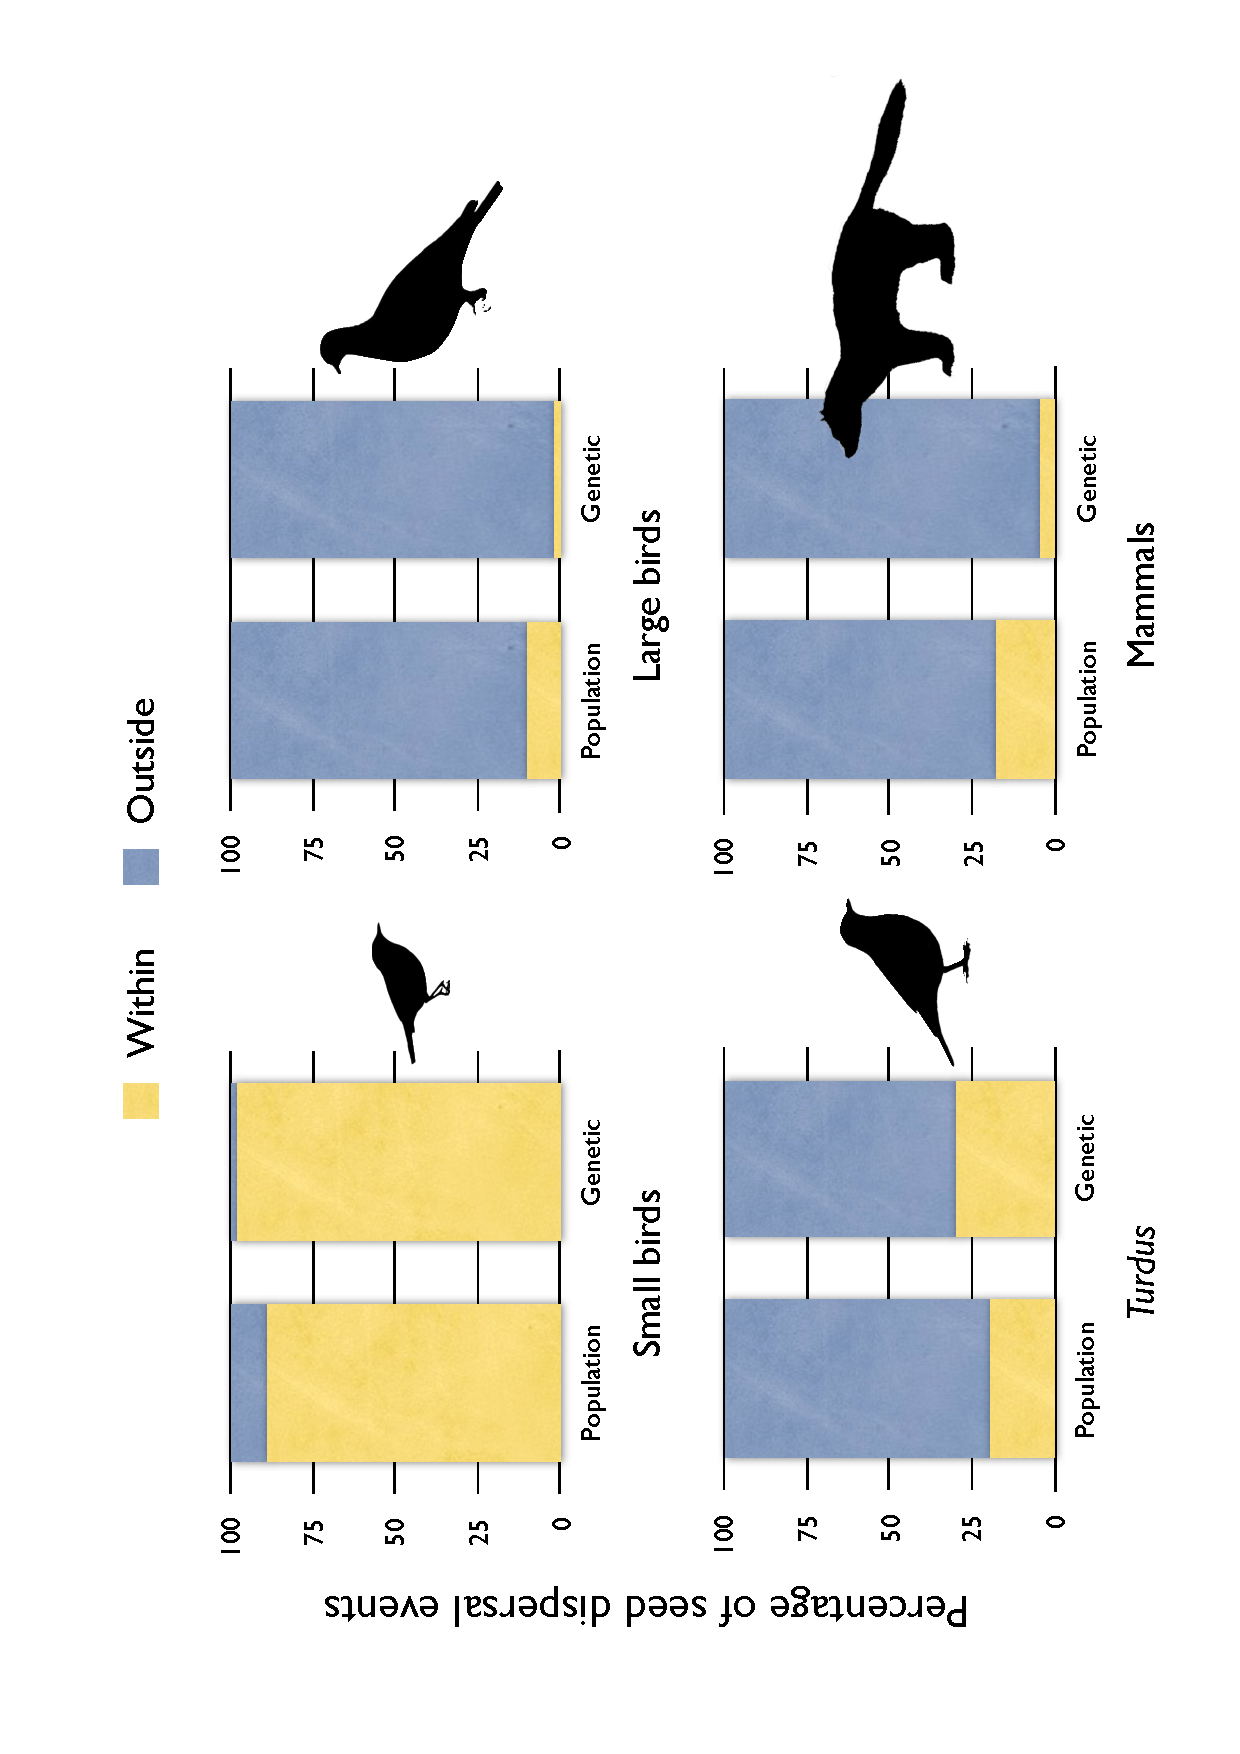
\includegraphics[height=26cm]{Fig4.pdf}}
%
%\caption{***}
\end{figure}

\newpage 

%%%%%%%%%%%%%%%%%%%%%%%%%%%%%%%%%%%%%%%%%%%%%%%%%%%%%%%%%%%%%%%%%%%%%%%%%%%%%%
\section*{Online Support Material and data accessiblity}

This review does not use new raw data, but includes some re-analyses of previously published material. All the original data supporting the paper, R code, supplementary figures, and summaries of analytical protocols is available at the author's GitHub repository (\texttt{https://github.com/pedroj/MS\_LDD}), with DOI: \texttt{\#/zenodo.\#}.
%%%%%%%%%%%%%%%%%%%%%%%%%%%%%%%%%%%%%%%%%%%%%%%%%%%%%%%%%%%%%%%%%%%%%%%%%%%%%%

\end{linenumbers}

%%%%%%%%%%%%%%%%%%%%%%%%%%%%%%%%%%%%%%%%%%%%%%%%%%%%%%%%%%%%%%%%%%%% MS NOTES
\begin{comment}
NOTES
% -------------- Crawford 21986 Heredity ------------------------------------
Sewall Wright's neighborhood model indicates that the area containing a panmictic unit within a continuous and uniform array of organisms can be 
estimated by $4\pir^2$ where a-2 is the parent-offspring dispersal variance measured around a zero  mean and relative to a single reference axis passing through the population.

% ---------------------------------------------------------------------------
Breeding unit size. Donor number is related to the size of the breeding unit (N individuals) as d= Np, where d is the number of different pollen parent genotypes represented in a maternal tree’s fruit crop and p is the expected proportion of trees in staminate phase at any given time. Assuming, conservatively, that individual trees reproduce asynchronously twice per year 6 and that staminate and pistillate flowering phases each last seven days 20, p is calculated to be 0.0712. Although these estimates could be effected by mosaicism 21 (the fusion of genetically distinct individuals), its frequency in the species examined here is low. 

Breeding unit area and radii. These parameters were calculated from paternity-analysis-based estimates of breeding unit size (Nˆdˆ; Table2) and the censused densities of adult, reproductively mature trees over 15 km2 BCI. Based on the long-term censuses of C. Handley and E. Kalko, 6, 108 and 20 adults of F. dugandii, F. obtusifolia and F. popenoei, respectively, are known to occur on BCI. Because these species exhibit little spatial aggregation over the area censused, these densities are assumed to be representative of forested areas surrounding BCI, a conservative assumption given that approximately one-third of the area within 10 km of BCI is occupied by Lake Gatun where figs are absent. Breeding unit radii estimate the distances pollen-bearing, female fig wasps routinely disperse in search of receptive host trees. Although actual breeding populations of figs may deviate substantially from the assumed circular distribution, alternative structures (elliptical,for example)increase estimated wasp dispersal distances. 

\begin{itemize}
\item Levin’s paternity pool concept.  Levin, D. A. The paternity pools of plants. Am. Nat. 132, 309–317 (1988).
\end{itemize}

[Burnham, K.P. \& Overton, W.S. Robust estimation of population size when capture probabilities vary among animals. Ecology 60, 927–936 (1979).]

\paragraph*{Genetic ‘neighborhood’}

For continuously distributed populations, Wright (1946) introduced the concept of a genetic ‘neighborhood’ that describes the local area within which most matings occur. In a two-dimensional land- scape, Wright’s neighborhood size (NS) is  

\$NS = 4pisigma\textasciicircum{}2 D\$  

where D is density (number of individuals per unit area) and \$sigma\$ (mean squared distance along one axis between birthplaces of parents and their offspring) is a measure of dispersal. \emph{NS} can be thought of as the number of reproducing individuals in a circle of radius \$2sigma\$. Assuming that dispersal is Gaussian, a circle of this size would include \textasciitilde{}87 \% of the potential parents of individuals at the center (Wright, 1946).

If the dispersal of an individual between place of birth and breeding site is essentially random, it resembles a "drunkards walk". It has the same distribution as passive diffusion, a two-dimensional normal distribution.

If this is true, dispersal distance can simply measured as the standard deviation, \$sigma\$, of the dispersal distribution.  A population "neighbourhood" can be defined approximately as a group of individuals who come from an area \$2sigma\$ wide.

[Strictly, \$sigma\$ is a valid measure of dispersal only if dispersal is exactly normally distributed. Many field studies have shown that dispersal is actually leptokurtic, i.e. most offspring breed very close to their parents, but some breed an enormous distance away. In practice, it doesn't much matter if dispersal is non-normal, provided it is not too extreme.]

% --------------------------------------------------------------------------
https://www.nceas.ucsb.edu/nceas-web/projects/2057/nceas-paper3/data/GFBoxB.html

Continuous populations can be modeled with the concepts of isolation by distance and neighborhood size\citep{Wright:1943aa,Wright:1946aa}. The former refers to the case that limited gene dispersal in continuous populations produces demes that are panmictic internally, but are isolated to some extent, from adjacent demes. Each group of reproducing individuals is the neighborhood, defined as the population of a region in a continuum, from which the parents of individuals born near the center may be treated as if drawn at random \citep{Wright:1969mb}. If distances between parents and offspring follow a normal distribution, the effective population size of the neighborhood will be:

$N_b= 4p \sigma^{2d}$

where $d$ is the density of adults per unit area and $\sigma$ is the variance in distance between birth and breeding sites. This is the basic model of ‘Isolation by Distance’ proposed by Wright  (1943, 1946). Under this type of model, migration (gene flow) is given by the variance in dispersal, and not by the proportion of the population that is composed of migrants (denoted $m$), as is the case with island models (Slatkin 1989).

For plants, gene flow may be accomplished by both seeds and pollen, so the variance may be decomposed to account for different patterns of seed and pollen dispersal, and to take into account the mating system (outcrossing rate, $t$). Thus, neighborhood size can be defined with the following equation (Crawford 1984) :

$N_b = 4p (\sigma^2_s + \frac{t \sigma^2_p}{2}) d (1 + t)$

where $\sigma^2_s$ is the variance in seed dispersal, $\sigma^2_s$ is the variance in pollen dispersal and $d$ is the density of potential parents.

Neighborhood size in plants can be estimated by marking pollen and seeds with fluorescent dyes, tags, or  marks. However, these methods do not measure effective pollen or seed movement, but they may be combined with genetic analysis to do so.  Individuals with a unique allele in a stand can provide valuable insight on seed movement \citep{Eguiarte:1993aa}.

%------ Levin & Kerster 1971 ------------------------------------------------
It has been shown that neighborhood size contracts under autogamy,as it does under dioecy or heteromorphic incompatibility if these morph ratios are disproportionate. Neighborhood size may expand under heteromorphic incompatibility or dioecy through enhanced pollen carry-over if the sex ratio is 1:1 and if the plants are insect-pollinated. 

\end{comment}
%%%%%%%%%%%%%%%%%%%%%%%%%%%%%%%%%%%%%%%%%%%%%%%%%%%%%%%%%%%%%%%%%%%%%%%%%%%%%
%----------------------------------------------------- SUPPLEMENTARY MATERIAL
%%%%%%%%%%%%%%%%%%%%%%%%%%%%%%%%%%%%%%%%%%%%%%%%%%%%%%%%%%%%%%%%%%%%%%%%%%%%%%
%% MS Draft Journal of Ecology Special Issue, Dispersal - SUPPL MATERIAL
%% Pedro - 07 June 2016
%----------------------------------------------------------------------------
%%%%%%%%%%%%%%%%%%%%%%%%%%%%%%%%%%%%%%%%%%%%%%%%%%%%%%%%%%%%%%%%%%%%% Headers
\documentclass[a4paper, 12pt]{article}
\usepackage{graphicx}
\usepackage[utf8]{inputenc}
\usepackage[a4paper]{geometry}
\usepackage{hyperref}
\pagestyle{plain}
\usepackage{amsmath,amssymb}
\usepackage{geometry}
\usepackage{lscape}
\usepackage{setspace}
\usepackage{verbatim}
\usepackage{graphicx}
\usepackage{epstopdf}
\usepackage{booktabs}
\usepackage{natbib}
\usepackage{longtable}
\usepackage{rotating}                                                                                     
\newcommand{\tab}{\hspace{5mm}}
\usepackage{tabularx} 
\usepackage[margin=10pt,font=small,labelfont=bf]{caption}
\usepackage[left]{lineno}
\usepackage{caption}
\DeclareGraphicsRule{.tif}{png}{.png}{`convert #1 `basename #1 .tif`.png}
\usepackage{fancyhdr} % This should be set AFTER setting up the page geometry
\pagestyle{empty}     % options: empty , plain , fancy
\renewcommand{\headrulewidth}{0pt} % customise the layout...
\lhead{{\tiny Jordano - What is long-distance dispersal?}}\chead{}\rhead{}
\lfoot{}\cfoot{\thepage}\rfoot{}
\usepackage{parskip}
\linespread{1.25}
%%%%%%%%%%%%%%%%%%%%%%%%%%%%%%%%%%%%%%%%%%%%%%%%%%%%%%%%%%%%%%%%%% Title page
\begin{document}


\title{\textbf{Supplementary Material}\\
\vspace{2cm}
What is long-distance dispersal? And a taxonomy of dispersal events \\
}

\author{Pedro Jordano$^{\dag}$}

\date{Sevilla, \today}
\maketitle


\begin{spacing}{1.0}
$^{\dag}$ {\small Integrative Ecology Group, Estaci\'on Biol\'ogica de 
Do\~nana, CSIC, Avda. Americo Vespucio, s/n, Isla de La Cartuja
E-41092 Sevilla, Spain.}\\


{\small \textit{Corresponding author:} Pedro Jordano. Integrative Ecology Group, Estaci\'on Biol\'ogica de Do\~nana, CSIC, Avda. americo Vespucio, s/n, E-41092 Sevilla, Spain. Email address: jordano@ebd.csic.es}\\

\textbf{Key words}: ***\\

{\small \textbf{Manuscript information: }** Words; ** Chars; ** Pages, * Figures; * Tables.}
\end{spacing}

\maketitle
\newpage

%-------------------------------------------------------------------- METHODS
\begin{linenumbers}

\section*{Methods}

\paragraph*{Species and Study Site.} The tree species we use as a case study to illustrate different types of dispersal events, \textit{Prunus mahaleb} (L.) (Rosaceae), is a shrub or small tree that produces fleshy fruits that are consumed by frugivores, who disperse seeds after regurgitating or defecating them. This species is frequently visited during July to mid-August by small- and medium-sized birds and carnivorous mammals that include fruits in their diets during late summer to winter \citep{Jordano:2000ft}. \textit{P. mahaleb} occurs in a patchy distribution at the regional scale, with relatively isolated populations consisting of dozens to hundreds of trees. Our study population included a total of 196 adult reproductive trees distributed over an area of 26 ha in patches of variable density. Other populations within 20 km exist as scattered patches of 10–150 trees, with some containing $\geqq$ 1,000 trees. The nearest population is 1.5 km away. Additional information on the study population and description of methodological apporaches is reported by \citet{Jordano:2007} and \citet{Garcia:2009do} and references therein.

\paragraph*{Sampling dispersed seeds.} 
To estimate the relative contribution of each dispersal vector to the different categories of dispersal events defined in Table 1, we first collected dispersed seeds, following different sampling schemes according to the functional group of dispersal vector. We used this grouping of frugivores giving the difficulties of resolving the identification of scats, pellets and regurgitated seeds down to species level just based on visual cues. We differentiated four major frugivore types: large carnivorous mammals (such as foxes, badgers, and stone martens); two species of medium- and large-sized frugivorous birds, mistle thrushes (\textit{T. viscivorus}), and carrion crows (\textit{C. corone}); and a pool of small-sized frugivorous birds, including warblers, redstarts, and robins \citep{Jordano:2007}. 

Seeds were collected in 1997–1999 and 2003–2005. The sampling schemes are described in detail elsewhere \citep{Jordano:2007,Garcia:2009do} and include a combination of seed traps and direct sampling of mammal feces along fixed transects. We haphazardly collected 130 samples of mammal feces during the \textit{P. mahaleb} fruit ripening period and recorded their location relative to potential source trees. Overall, we genotyped 167 seeds from 20 fecal samples. Most samples were from red fox (\textit{Vulpes vulpes}) and stone marten (\textit{Martes foina}); some ( 10 samples) were from badger (\textit{Meles meles}) \citep{Jordano:2007}.

In addition we sampled directly the pellets of large corvids (\textit{Corvus corone}) and from \textit{Turdus viscivorus}, the latter by direct sampling beneath pine trees and scats from seed traps \citep[see ][ for details]{Jordano:2007}. Finally, a seed sample directly from seed traps included seeds dispersed by small- and medium-sized passerines, such as \textit{Phoenicurus ochruros}, \textit{Turdus merula}, \textit{Erithacus rubecula}, \textit{Sylvia communis}, \textit{Sylvia atricapilla}, etc. \citep{Jordano:2007}. The total seed sample thus consisted of seed endocarps collected from the seed traps (mostly small passerines) ($n= $465), mammal scats ($n= $167), and \textit{C. corone} pellets ($n= $23) \citep[see Table 1 in ][]{Jordano:2007}. 

\paragraph*{Seed genotyping.} 
We used material described in \citet{Jordano:2007}, and genotyping methods described in detail in previous work \citep{Godoy:2001,Garcia:2007he,Garcia:2009do}. Briefly, we used a set of 10 polymorphic microsatellite markers (simple DNA sequence repeats) \citep{Godoy:2001} to obtain the multilocus genotypes of both of the adult trees (candidate source trees from the study population) and the sample of seed endocarps. Given that all adult trees in the population had a distinct multilocus genotype, an unambiguous assignment of each seed to its source tree could be made. When a full match between the endocarp genotype and any of the adult-tree genotypes in the population was not possible, we assumed that the seed came from another population. To assess the effect of genotyping errors, we reexamined the exclusion of genotypes due to a single locus mismatch, two loci mismatches, etc. At the analysis level, any exclusion of identity between a seed and a potential mother tree based on mismatches of only one or two loci was rechecked. We used GIMLET software \citep{Valiere:2002fo} to find the matching adult multilocus genotype for each endocarp with eight or more loci successfully typed. Because each seed belonged to one of the four groups of dispersers, we could thus derive the relative contribution of each frugivore group to different classes of seed dispersal events and to seed immigration.

\paragraph*{Contribution of dispersal vectors to types of dispersal events.} 
We considered each dispersed seed as an independent replicate, because each represented a dispersal event from the perspective of plant population genetics, i.e., an independent "arrival" event resulting from the dispersal process mediated by the frugivore. 

Once the maternal source tree of each individual seed was identified (or its provenance from outside the study population determined) we assessed the dispersal distance and grouped the seeds separately as coming from trees located within or outside the population. In addition, for seeds originating from local trees we determined whether dispersal distances were $\geqq$ 45 m to sort out $LDD_{loc}$ dispersal events from $SDD_{loc}$ events. All the events involving immigrant seeds were considered $LDD_{ss}$ by definition, given that the neighborhood size was very reduced (radius= 0.045 km) relative to the geographic limits of the study population (maximum length for a within-population dispersal event: 1220 m)\citep{Garcia:2009do}. Along this reasoning, $LDD_{neigh}$ events were considered non-existent in this particular case study given that neighborhood size area was smaller than the population area.

\end{linenumbers}
\newpage

%%%%%%%%%%%%%%%%%%%%%%%%%%%%%%%%%%%%%%%%%%%%%%%%%%%%%% Supplementary Material
%------------------------------------------------------------------- Table S1
\begin{landscape}
\begin{table}
  \caption*{Table S1. Summary of neighborhood area sizes and estimated neighborhood radius for tree species with different combinations of dispersal modes. Data from \citet{Nason:1998aa,Smouse:2001aa,Garcia:2005fu,Garcia:2007he,Dutech:2005fk} and present study.}
  \vspace{0.5cm}
    \begin{tabular}{lllccc}
        \hline \\
     Species                & Pollinator  & Seed disperser & Density ($ha^{-1}$) & Breeding unit ($km^2$) & Radius (km) \\\\ \hline \\
    \textit{Ficus dugandii}          & Fig wasp    & Vertebrates    & 0.004          & 631.7               & 14.2        \\
    \textit{Ficus obtusifolia}       & Fig wasp    & Vertebrates    & 0.072          & 105.9               & 5.8         \\
    \textit{Prunus mahaleb}          & Bees, flies & Vertebrates    & 0.003          & 0.87                & 0.042       \\
    \textit{Frangula alnus}          & Bees, flies & Vertebrates    & 0.0004         & 0.45                & 0.013       \\
    \textit{Astrocaryum mexicanum}   & Beetle      & Vertebrates    & 1364.0         & 0.011               & 0.06        \\
    \textit{Calophyllum longifolium} & Bees        & Vertebrates    & 0.28           & 1.241               & 0.629       \\
    \textit{Platypodium elegans}     & Bees        & Wind           & 0.78           & 0.866               & 0.525       \\
    \textit{Quercus lobata}          & Wind        & Vertebrates    & 3.0
      & 0.072               & 0.719       \\ 
    \textit{Quercus alba}            & Wind        & Vertebrates    & 92.8
      & 0.0009              & 0.017       \\ 
    \textit{Cedrus atlantica}        & Wind        & Wind           & 61.7           & 0.151               & 0.22        \\
   \textit{Fraxinus americana}       & Wind        & Wind           & 24.7           & 0.008                & 0.05        \\
    \textit{Pseudotsuga menziesii}   & Wind        & Wind           & 25.0           & 0.078               & 0.158       \\\\
\hline
    \end{tabular}
\end{table}
\end{landscape}
\newpage 

%------------------------------------------------------------------ Figure S1
\begin{figure}[htbp]
\centerline{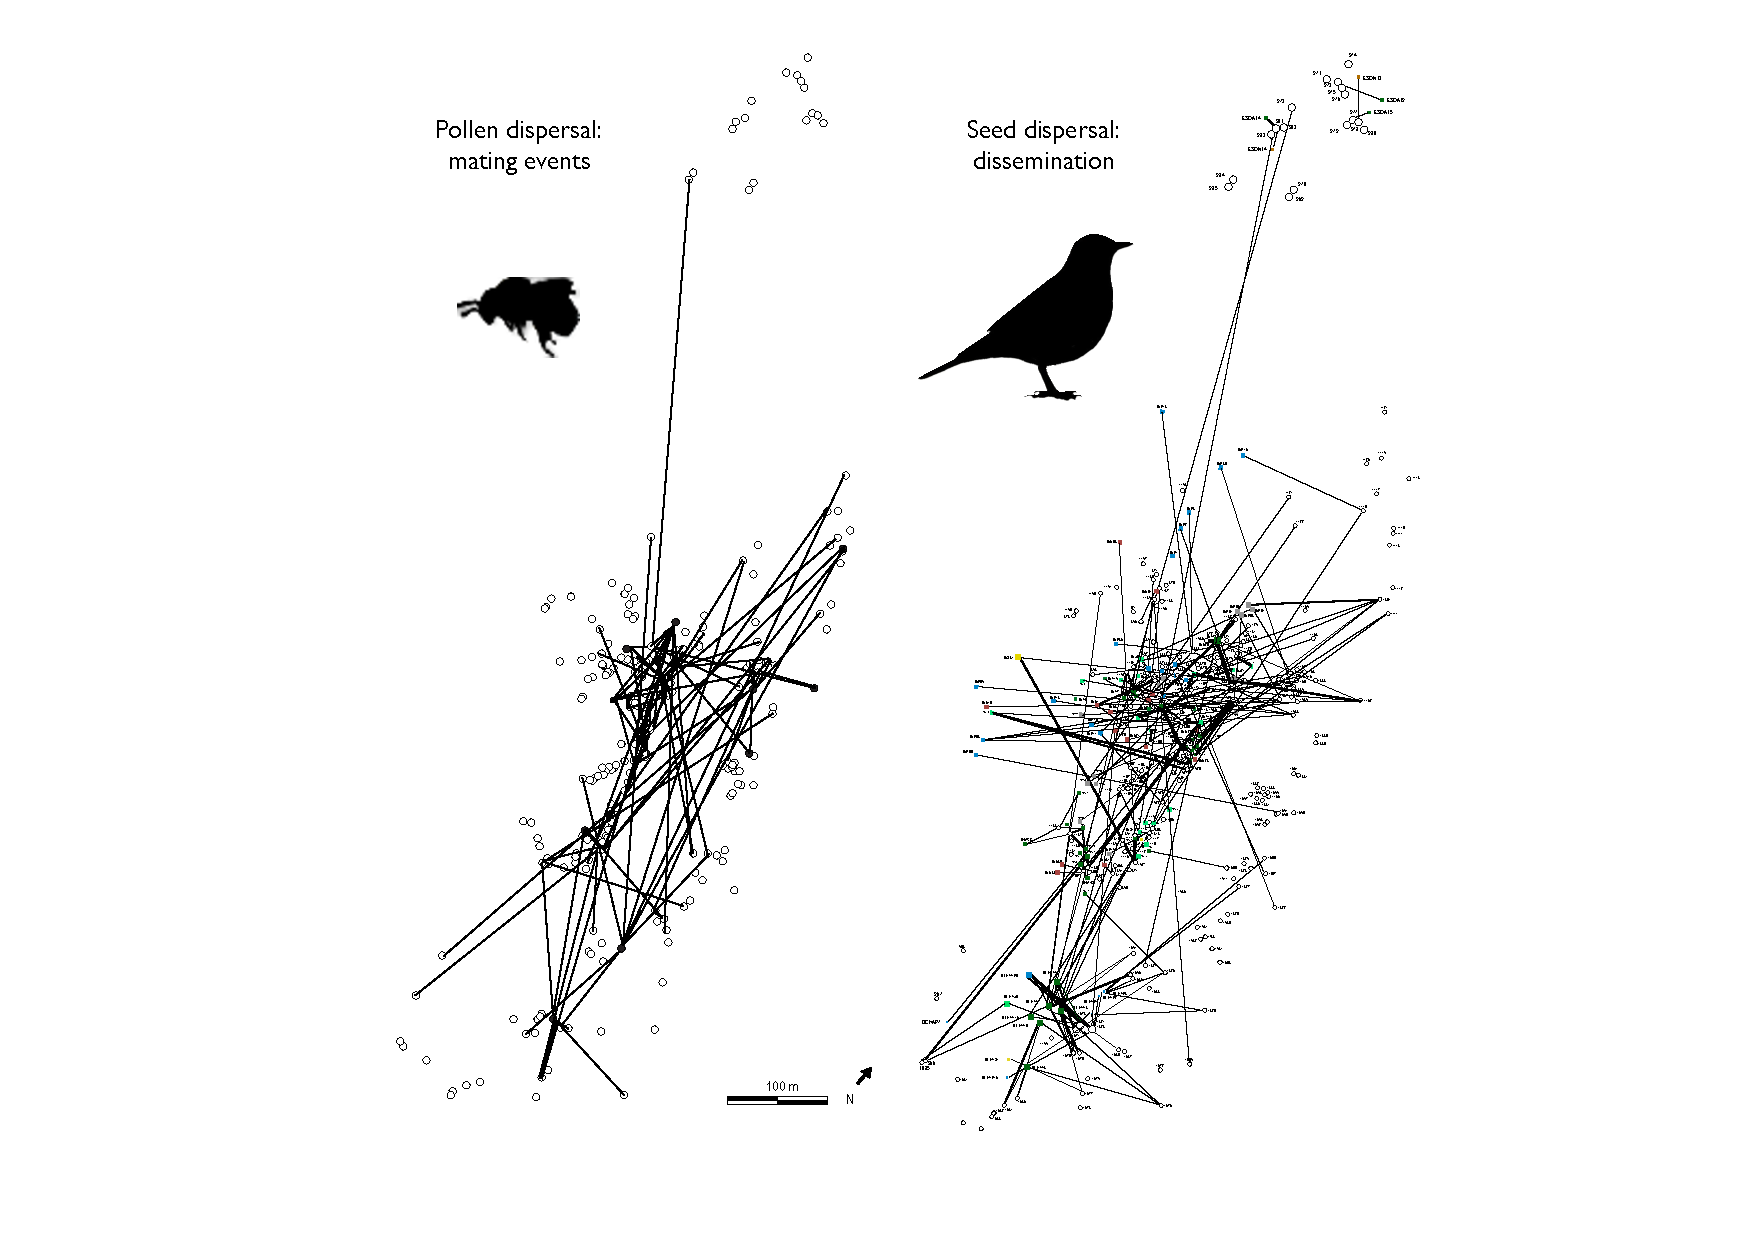
\includegraphics[height=21cm]{FigS1.pdf}}
%
\caption*{Figure S1. Dispersal events for pollen (left) and seeds (right) traced for \textit{Prunus mahaleb} trees (white dots). All the adult, reproductive, trees in the population are mapped. Lines indicate mating events of pollen dispersal among trees (left) or seed dissemination events from source fruiting trees to seed traps (squares; right). Line thickness is proportional to the number of events recorded.}
\end{figure}

\newpage 

%------------------------------------------------------------------ Figure S2
\begin{figure}[htbp]
\centerline{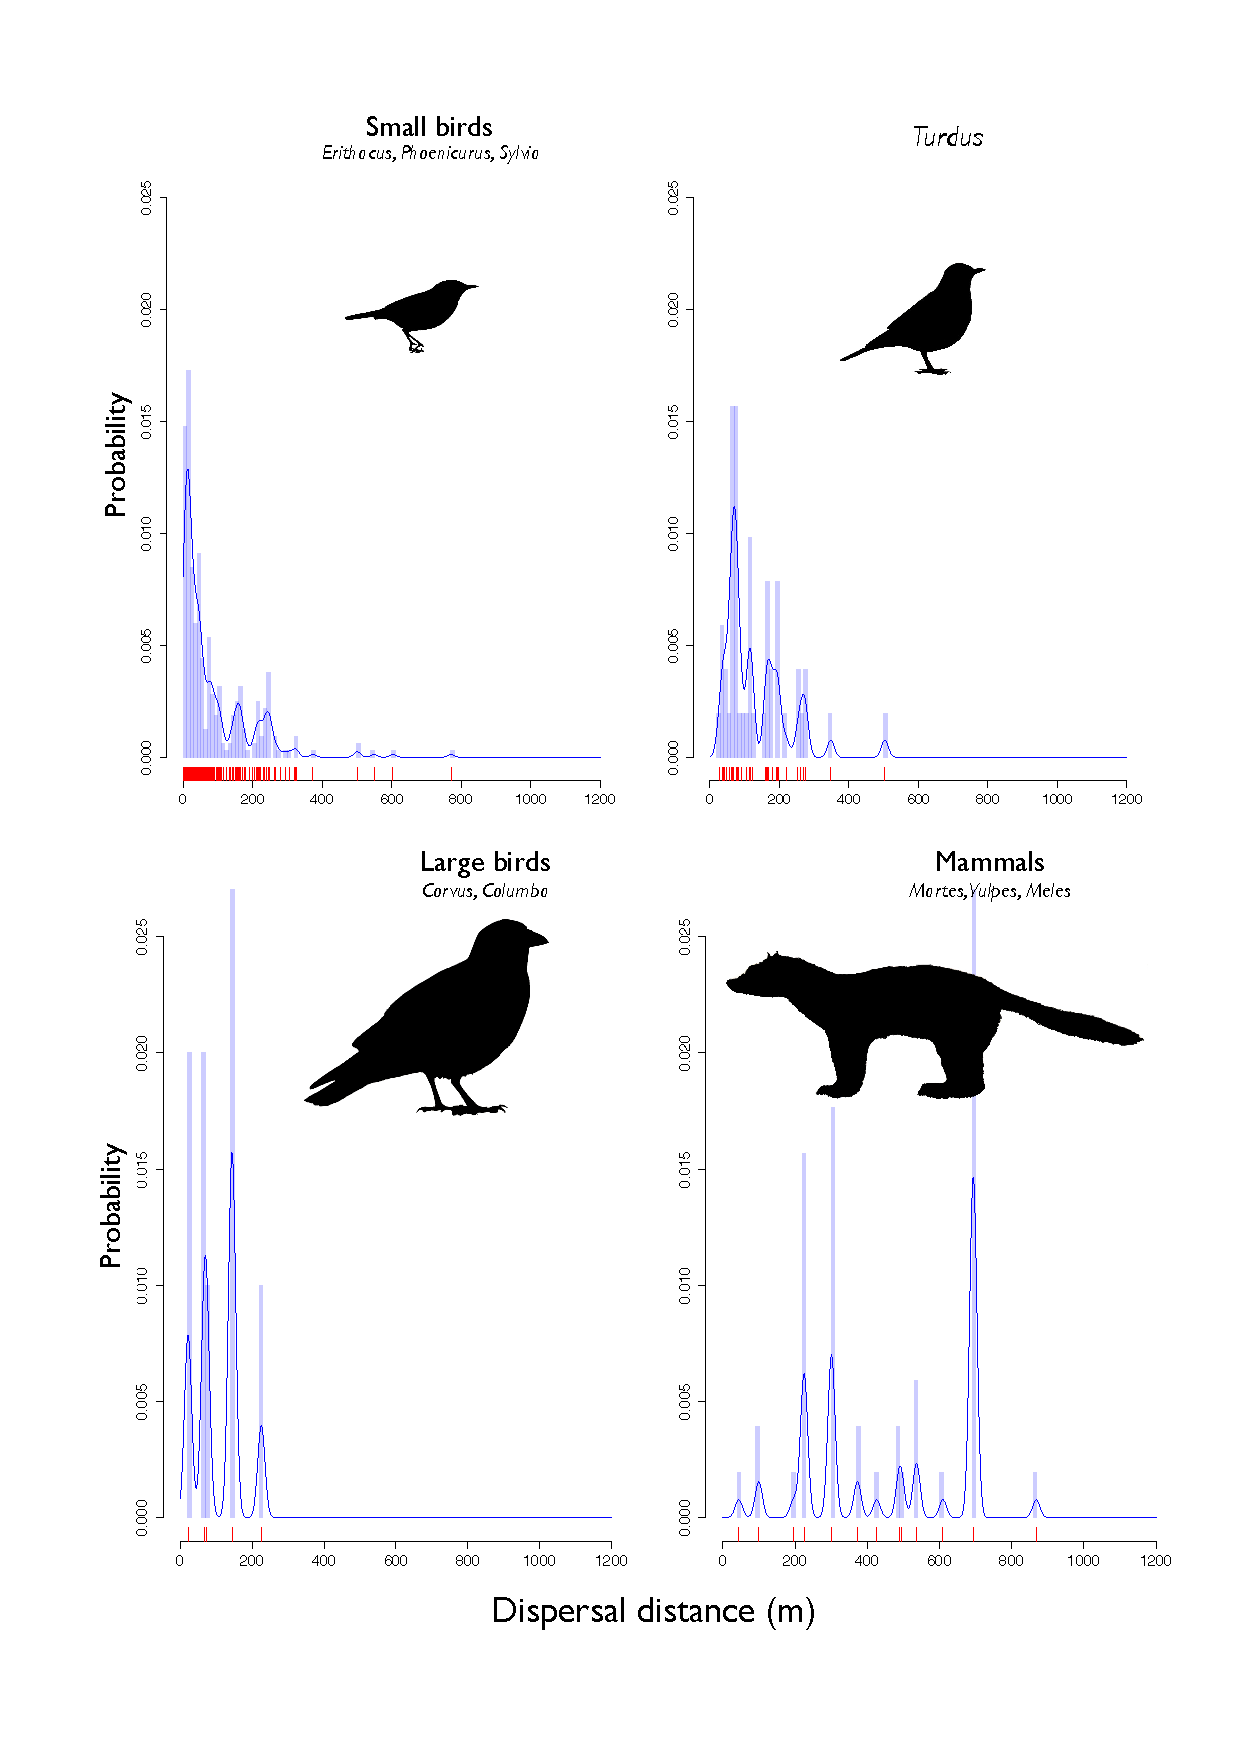
\includegraphics[height=22cm]{FigS2.pdf}}
%
\caption*{Figure S2. Differential contributions of functional groups of frugivores to the short- ($SDD_{loc}$) and long-distance ($LDD_{loc}$) local seed dispersal events for \textit{Prunus mahaleb}.}
\end{figure}

\newpage 
\newpage 

%\section*{References}
%%%%%%%%%%%%%%%%%%%%%%%%%%%%%%%%%%%%%%%%%%%%%%%%%%%%%%%%%%%%%%%%%%%%%%%%%%%%% References
%%% Unnumbered Literature Cited
\bibliographystyle{bes}        %Compile with bes.bst style file
\bibliography{MS_BES}

%%%%%%%%%%%%%%%%%%%%%%%%%%%%%%%%%%%%%%%%%%%%%%%%%%%%%%%%%%%%%%%%%%%%%%%%%%%%%
	
\end{document}

%%%%%%%%%%%%%%%%%%%%%%%%%%%%%%%%%%%%%%%%%%%%%%%%%%%%%%%%%%%%%%%%%%%%%%%%%%%%%

\end{document}
